\section{Extensible Authentication Protocol}
\label{section:eap}
Our protocol should be implemented using the EAP framework, lets overview how the protocol works and how we were to implemented a new EAP method.


%EAP - PROTOCOL IN DETAIL

\subsection{Overview}
Extensible Authentication Protocol \cite{aboba2004extensible} (EAP) is a general purpose authentication framework, designed for network access authentication, where IP might not be available. 
It runs directly over the data link layer such as PPP  \cite{simpson1994rfc1661} and IEEE 802.

EAP defines a set of messages that support negotiation and execution of a variety of authentication protocols.

EAP is a two-party protocol between a \textit{peer} and an \textit{authenticator} at the each end of a link. The terms \textit{peer} and \textit{authenticator} are EAP terminology.
In the protocol the peer is authenticating with the authenticator.

\subsection{Messages}
The peer and the authenticator communicate by exchanging \textit{EAP messages}.
The protocol starts with the authenticator sending a message to the peer, they keep exchanging messages until the authenticator can either authenticate the peer or not.

Messages are exchanged in a lock-step manner, where an authenticator sends a message and the peer responds to it. 
The authenticator dictates the order of messages, meaning it can send a message at any point of communication, as opposed to the peer, which can only respond to messages from the authenticator.
Any messages from the peer not in a response to the authenticator are discarded.

\begin{figure}[h]
	\centering
	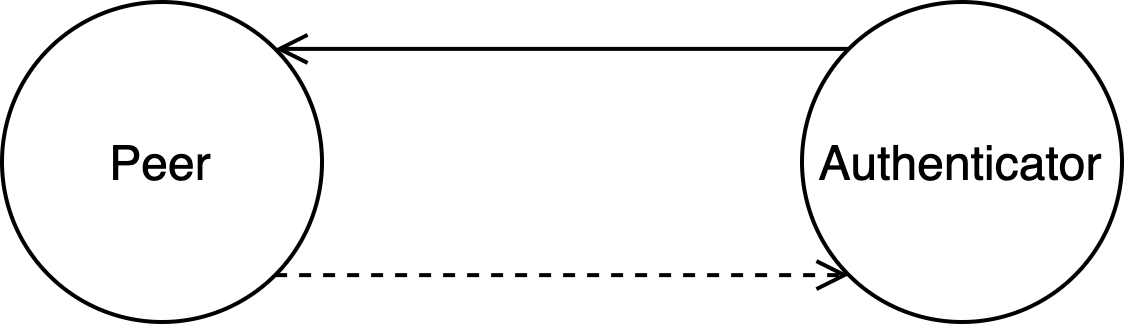
\includegraphics[width=8cm]{images/eap-messages}
	\caption{Peer and Authenticator Communication}
	\label{fig:eap-messages}
\end{figure}

\subsubsection{EAP Message Structure}
Messages are composed of fields, each field length is multiple of an octet of bits.
Each field type has a special purpose in EAP.

\begin{center}
	\begin{tabular}{|c|c|c|c|c|c|}
		\hline
		Length (Octets) & 1 & 1 & 2 & 1 & $n \le 2^{16}$\\
		\hline
		Field Type & Code & Identifier & Length & Type & Type-Data\\
		\hline
	\end{tabular}
\end{center}

%TODO: EAP Packet with table

\subsubsection{Code Field}
The code field determines who the packet is intended for and how or even should the recipient respond.

\begin{description}
	\item[Request]\textit{Code 1}. Messages sent by the authenticator to the peer.
	\item[Response]\textit{Code 2}. Messages sent by the peer to the authenticator as a reply to a \textit{request} message.
	\item[Success]\textit{Code 3}. Sent by the authenticator, after the peer is successfully authenticated. The peer doesn't have to respond to the message.
	\item[Failure]\textit{Code 4}. Sent by the authenticator, if the peer cannot be authenticated. The peer doesn't have to respond to the message.
\end{description}

\subsubsection{Identifier Field}
The identifier field is used to match request and response messages, each response message needs to have the same identifier as the request.
The authenticator will discard response messages that don't have a matching identifier with the current request.
The peer does not re-transmit response message, but relies on the authenticator to re-transmit a request message after some time if the matching response is lost.

\subsubsection{Length Field}
The length field determines the total size of the EAP message. Because EAP provides support for generic authentication methods, the final length of the messages is variable.
The length of the Type-Data field is entirely dependent on the authentication method used.

%EAP - METHODS

\subsubsection{Type and Type-Data Field}
The \textit{type} field determines how the message should be processed and how to interpret the \textit{type-data} field.
Most message types represent authentication methods, except four special purpose types.

The \textit{type} used is determined by the authenticator when sending the request message. The response message from a peer needs to be of the same \textit{type} as the request, except in cases where that \textit{type} is not supported by the peer.

\begin{description}
	\item[Identity] \textit{Type 1}. Used to query the identity of the peer. The type is often used as an initial message from the authenticator the peer, however its use is entirely optional and EAP methods should rely on method-specific identity queries.
	
	\item[Notification]\textit{Type 2}. Used to convey an informative message to the peer, by the authenticator. Usage of this type is entirely optional.
	\item[Nak]\textit{Type 3}. Used only as a response to a request, where the desired type is not available.
	The peer includes desired authentication methods, indicated by their type number.
	This type is also referred to as Legacy Nak, when compared to \textit{Expanded Nak} (sub-type of the Expanded Type).
	\item[Expanded Type] \textit{Type 254}. 
	Used to expand the space of possible message types beyond the original 256 possible types.
	The expanded type \textit{data field} is composed from a \textit{Vendor-ID} field, \textit{Vendor-Type} and the type data.
	\bigskip
	\begin{center}
		\begin{tabular}{|c|c|c|c|c|c|}
		\cline{2-5}
		\hline
		Length (octets) & & 3 & 4 & n\\
		\hline
		Type Field & ... & Vendor-ID & Vendor-Type & Vendor-Type Data\\
		\hline
		\end{tabular}
	\end{center}
	\bigskip
	A peer can respond to an unsupported request type with an \textit{expanded nak}, if he desires to use an EAP method supported with the expanded type.
	\item[Experimental] \textit{Type 255}. This type is used for experimenting with new EAP Types and has not fixed format.
\end{description}

\subsubsection{Authentication Methods}
The remaining types correspond to different authentication methods.
In IANA \cite{joseph2004eap} 49 authentication methods have been assigned type numbers.
The original RFC \cite{aboba2004extensible} already assigned 3 authentication protocols.

\begin{description}
	\item[MD5-Challenge] \textit{Type 4}. An EAP implementation of the \cite{simon2008eap} PPP-CHAP protocol.
	\item[One-Time Password] \textit{Type 5}. An EAP implementation of the \cite{haller1998one} one-time password system.
	\item[Generic Token Card] \textit{Type 6.} This type facilitates various challenge/response \textit{token card} implementations.
\end{description}

Some other notable examples are EAP-TLS \cite{simon2008eap}, EAP-PSK \cite{bersani2007eap}.
EAP SRP-SHA1 \cite{carlson135eap} is especially interesting as it uses a zero-knowledge protocols to verify the peers secret.

\subsection{Pass-Through Behaviour}
An authenticator can act as a \textit{Pass-Through Authenticator}, by using the authentication services of a \textit{backend authentication server}.
In this mode of operation the authenticator is relaying the EAP messages between the peer and the backend authentication server.
For example, in IEEE 802.1x the authenticator communicates with a RADIUS server \cite{congdon2003ieee}.

\paragraph{IEEE 802.1x}

Is a port based network access control standard for LAN and WLAN.
It is part of the IEEE 802.11 group of network protocols.

IEEE 802.1x defines an encapsulation of EAP for use over IEEE 802 as EAPOL or "EAP over LANs".
EAPOL is used in widely adopted wireless network security standards WPA2. 
In WPA2-Enterprise, EAPOL is used for communication between the supplicant and the authenticator.

With WPA2-Enterprise, the authenticator functions in a pass-through mode and uses a RADIUS server to authenticate the supplicant.
EAP packets between the authenticator and the authentications server (RADIUS) are encapsulated as RADIUS messages \cite{aboba2003radius, chen2005extensible, congdon2003ieee}